\clearpage
\subsection{Constant} % (fold)
\label{sub:constant}

A Constant is just like a \nameref{sub:variable}, but its value cannot be changed. Constants are declared within the Program, and given a value when they are created. Once they are created the value within the Constant cannot be changed. This is useful for data where you do not want the value changing during the program's execution.

\begin{figure}[h]
   \centering
   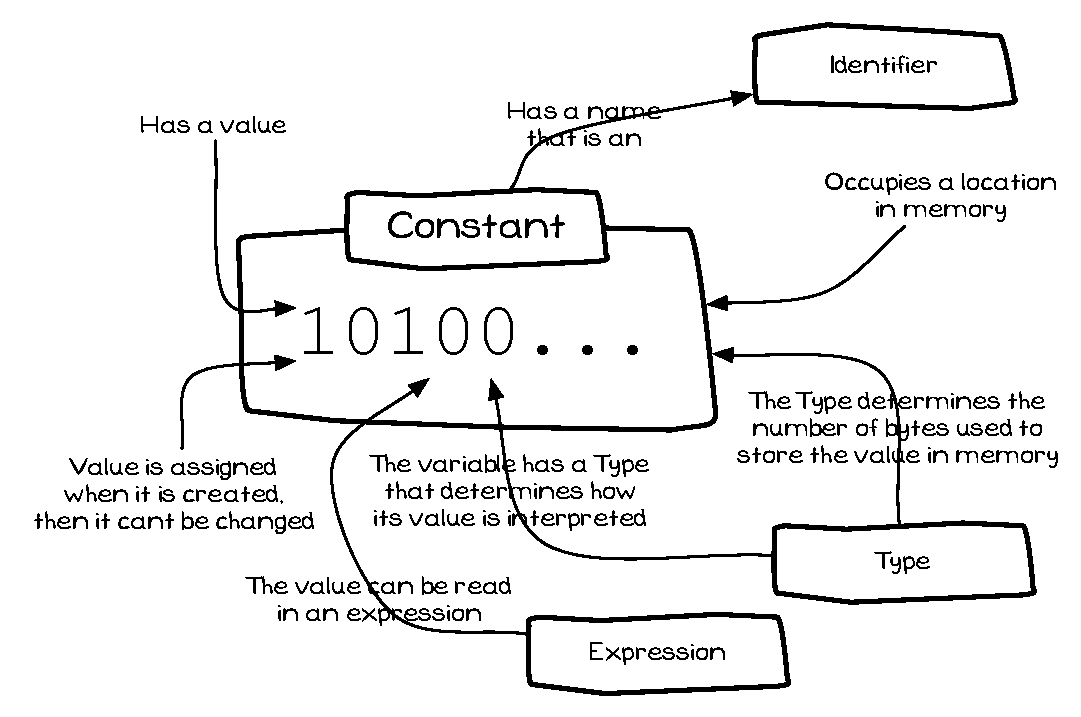
\includegraphics[width=\textwidth]{./topics/storing-using-data/diagrams/Constant} 
   \caption{Constants have a value that cannot be changed}
   \label{fig:constants}
\end{figure}

\mynote{
\begin{itemize}
  \item A Constant is an \textbf{artefact}. You can create Constants in your Program to store values that must not change.
  \item A Constant is similar to a \nameref{sub:variable}, they have a...
  \begin{itemize}
    \item \textbf{Name} that is used to access them.
    \item \textbf{Value} that can be read in an Expression.
    \item \textbf{Type} that determines how their data is interpreted.
  \end{itemize}
  \item You \textbf{read} \emph{values} of Constants in Expressions.
  \item Constants are useful for data you do not want to change during the program. 
  \item The name of the Constant is an \nameref{sub:identifier}.
  \item The Constant's name should reflect the value it is storing.
\end{itemize}
}

% subsection constants (end)